%%%%%%%%%%%%%%%%%%%%%%%%%%%%%%%%%%%%%%%%%%%%%%%%%%%
%
%  New template code for TAMU Theses and Dissertations starting Fall 2012.  
%  For more info about this template or the 
%  TAMU LaTeX User's Group, see http://www.howdy.me/.
%
%  Author: Wendy Lynn Turner 
%	 Version 1.0 
%  Last updated 8/5/2012
%
%%%%%%%%%%%%%%%%%%%%%%%%%%%%%%%%%%%%%%%%%%%%%%%%%%%
%%%%%%%%%%%%%%%%%%%%%%%%%%%%%%%%%%%%%%%%%%%%%%%%%%%%%%%%%%%%%%%%%%%%%%
%%                           SECTION V
%%%%%%%%%%%%%%%%%%%%%%%%%%%%%%%%%%%%%%%%%%%%%%%%%%%%%%%%%%%%%%%%%%%%%


\chapter{\uppercase{Experiments \& Results}}
To verify the idea proposed in this thesis, we setup environments, develop SAC framework and run some typical seismic applications on cluster in PVAMU cloud computing lab. There are three main layers in SAC: low-level runtime envrionment, SAC framework as middleware and application development interface at up-level. 

\section{Experiments Environment Setup}

The cluster used for conducting experiments consists of 26 nodes, in which one is management node, another is storage node used for managing disk array and other 24 nodes are computation nodes. Each node in such cluster was equipped with Intel Xeon E5-2640 Sandy Bridge CPU (2.5GHz, 12 Cores or 24 Cores with Hyperthreading support), 64GB DDR3 memory and are inter-connected with 1GB ethernet. Each node has its own local disk, and also could access disk array through NFS. Following the architecture stated in previous charpter, we install CentOS 6.5 (Distributed by Redhat) and Oracle JDK 1.8.0\_40 on each node. Hadoop 2.2.0, Spark 1.2.1 and other related libraries are also installed on each node. In configuration of Hadoop, management node was configured as NameNode and other 24 computation nodes as DataNodes. It is similiar in Spark: management node is Master and other computation nodes are Workers. Cassandra was installed on all 24 computation nodes and the first four nodes was selected as seed nodes.

The public sample seismic dataset Penobscot \cite{PenobscotData} was selected as experiment data. The original format of Penobscot dataset is SEGY, and to make it easily processed with Spark, we transfer it into two files: one xml file that saves meta data, and aonther 3D data file with dimension size of 600x481x1501 stores actual data samples. The volume size of original data file is about 1.7GB, which is not big enough comparing with data set currently used in oil\&gas industry, so we use it synthesize a new 100GB file for verifying algorithms and models on SAC. Both xml file and data file are stored on HDFS, so that every node could access them and utilize data locality. The intermediate results are stored in Cassandra basing on requirement and final result are persisted on HDFS. 

\section{Application Development Platform}

As stated in previous charpter, user could create new application that calls APIs provide by SAC framework, but another more convenient way is using Web interface provide by SAC platform. In web development interface, SAC platform provides four main components: Projects, Data Sets, Jobs and Workflow. The typical flow is listed below:

\begin{enumerate}
  \item Create a project or open an existing project. While create new project, user need to select template as shown in Figure \ref{NewProject}.
  \item Edit codes, compile project and fix erros until compiling successfully as shown in Figure \ref{Programming}.
  \item Select data set(s) as input parameter as shown in Figure \ref{DataSet}.
  \item Configure runtime environments and submit job to Spark Jobserver as shown in Figure \ref{Runtime}.
  \item Check job status and view results after job finished.
\end{enumerate}

%%%%%%%%%%%%%%%%%%%%%%%%%%%%%%%%%%%%%%%%%%%%%%%%%%%%%%%
\begin{figure}[H]
%\centering
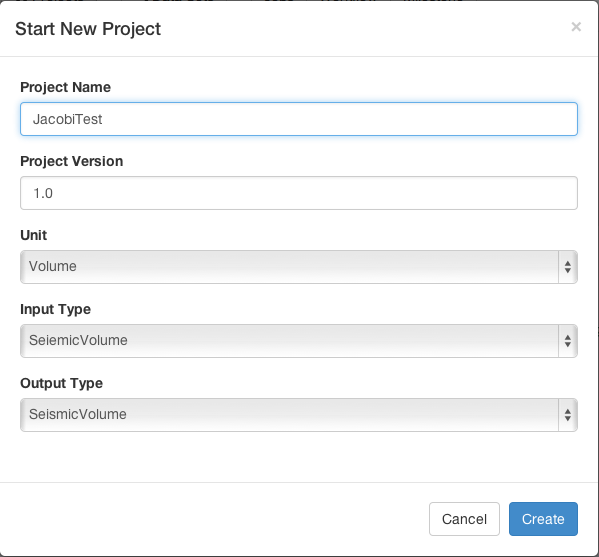
\includegraphics[scale=.60]{figures/NewProject.png}
\caption{Configure Template on Creating New Project}
\label{NewProject}
\end{figure}
%%%%%%%%%%%%%%%%%%%%%%%%%%%%%%%%%%%%%%%%%%%%%%%%%%%%%%%

%%%%%%%%%%%%%%%%%%%%%%%%%%%%%%%%%%%%%%%%%%%%%%%%%%%%%%%
\begin{figure}[H]
\centering
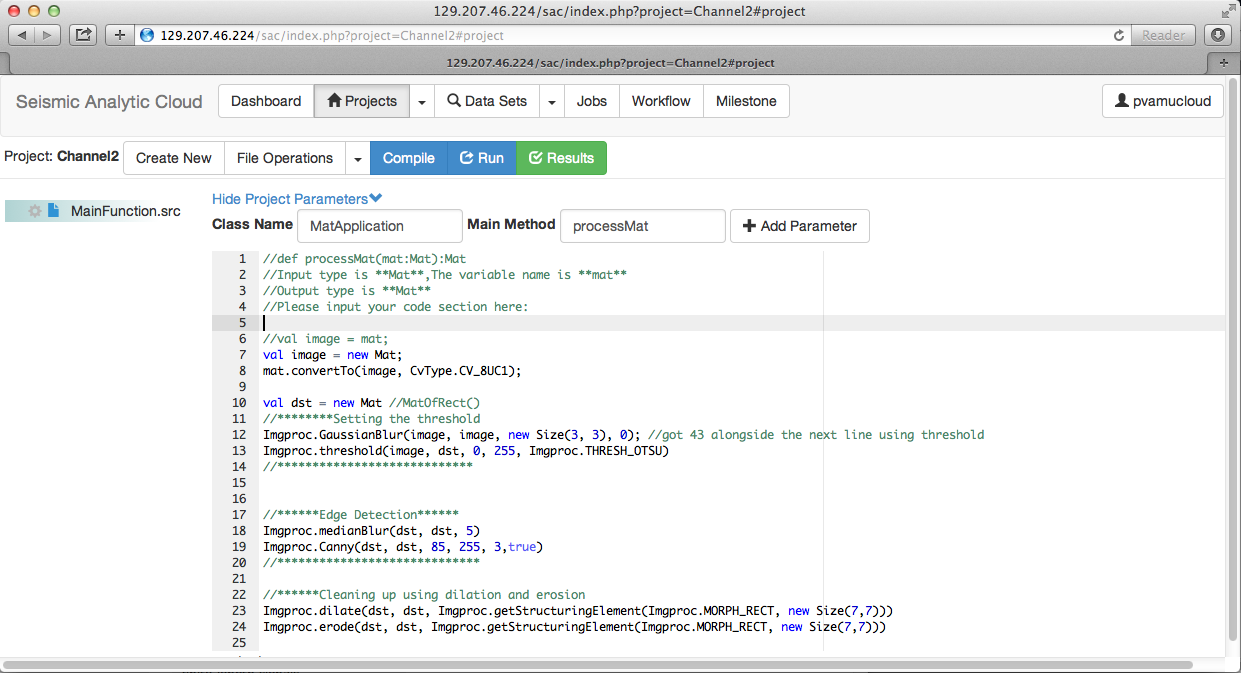
\includegraphics[scale=.35]{figures/Programming.png}
\caption{Programming and Running on Web Interface}
\label{Programming}
\end{figure}
%%%%%%%%%%%%%%%%%%%%%%%%%%%%%%%%%%%%%%%%%%%%%%%%%%%%%%%


%%%%%%%%%%%%%%%%%%%%%%%%%%%%%%%%%%%%%%%%%%%%%%%%%%%%%%%
\begin{figure}[H]
\centering
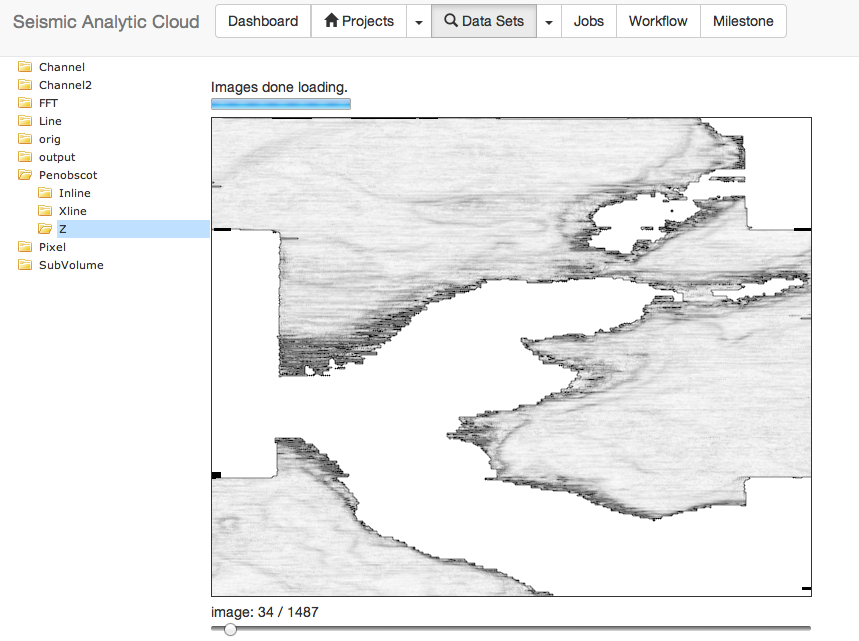
\includegraphics[scale=.45]{figures/DataSet.png}
\caption{Seismic Dataset Preview}
\label{DataSet}
\end{figure}
%%%%%%%%%%%%%%%%%%%%%%%%%%%%%%%%%%%%%%%%%%%%%%%%%%%%%%

%%%%%%%%%%%%%%%%%%%%%%%%%%%%%%%%%%%%%%%%%%%%%%%%%%%%%%%
\begin{figure}[H]
\centering
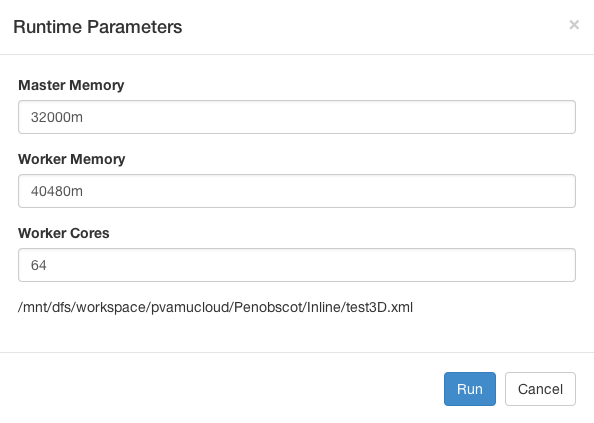
\includegraphics[scale=.60]{figures/Runtime.png}
\caption{Specify runtime parameters}
\label{Runtime}
\end{figure}
%%%%%%%%%%%%%%%%%%%%%%%%%%%%%%%%%%%%%%%%%%%%%%%%%%%%%%

%A table example is going to follow.
\begin{table}[H]
\centering
\caption{Provided UFuncs by ScalaNLP Breeze}
%\begin{tabular}{|p{4cm} |p{8cm} |}
\begin{tabular}{|l|l|}
\hline
Elementwise UFuncs & \shortstack[l]{exp, log, log1p, sqrt, \\sin, cos, tan, asin, acos, atan,\\sinh, cosh, tanh, asinh, acosh, atanh, \\floor, ceil, round, rint, signum, \\abs, isOdd, isEven,sigmoid} \\ 
\hline
Operator UFuncs &  \shortstack[l]{OpAdd: a + b, OpSub: a - b, OpMulMatrix: a * b, \\OpMulScalar: a :* b, OpSolveMatrixBy: a \textbackslash\ b,\\ OpMulInner: a dot b, OpNeg: -a, OpEq: a :== b,\\OpNe: a :!= b, OpLT: a :\textless\ b, OpLTE: a :\textless= b,\\OpGT: a :\textgreater b, OpGTE: a :\textgreater= b, \\OpAnd: a \& b, OpOr: a \textbar\ b, OpNot: !a } \\
\hline
Reduction UFuncs & \shortstack[l]{sum, product, softmax, any, all, \\min, max, argmin, argmax, \\norm, normalize, argsort, argtopk, \\mean, variance, stddev, meanAndVariance }\\
\hline
\end{tabular}
\label{tab:BreezeUFuncs}
\end{table}
%%%%%%%%%%%%%%%%%%%%%%%%%%%%%%%%%%%%%%%%%%%%%%%%%%%%%%

\section{Case Study}
The main characteristics of SAC are productivity, performance, usability and scalability. To prove them, some typical applications in seismic data processing are selected to run on SAC. As for usability and productivity, we will show some codes snippet need to be implemented by end user. As for the performance, executation time of both sequential codes and parallel codes on Spark are compared to get speedup factor, and for scalability, we will configure the running environment with different cores and analyse changing of executation time. To cover more seismic applications, we select four applications as test cases: Calculactor, Transformation, Statistics Functions and Jacobi Stencil codes.

\subsection{Calculactor}
Calculactor should be the most common used tool in scientific computation. Basic arithmetic operations are easy implemented on normal data, but for big data, the situation is totally different. There are already some commerical and free seismic calculators such as Calculactor in Petrel, Seismic Toolkit listed in \cite{SeismicCalculator} etc. All these seismic calculator are software running on PC, so the performance is bad for handling big seismic data, and most of them even could handle big data. Calculactor designed in SAC is mainly focus on handling big data, in which data is distributed on different nodes and run arithmetic functions in parallel. Most functions in calculator are applied on pixel or sample, and each pixel is a Float type in Scala, so all built-in operator could be used on pixel data. The more convenient way to implement such algorithms are use operators and operations provided by Breeze. For trace or line template in SAC, the data types of input and output are DenseVector and DenseMatrix. ScalaNLP Breeze provide many Universal Functions (UFunc) that can operate on scalars, vectors, matrices, counters with little effort \cite{BreezeUFunc}. All Elementwise UFuncs from scala.math such as exp, log and trigonometric functions etc., and Operator UFuncs such as basic arithmetic, equality and comparison and boolean operations could be applied to DenseVector and DenseMatrix. Table \ref{tab:BreezeUFuncs} shows the functions and operators provided by ScalaNLP Breeze. List \ref{ScalaCode2Line} shows the sample codes of template for processing two Inlines and generate one output Inline.  
\lstset{language=Java,frame=single}
\begin{lstlisting}[float,caption=Sample codes of arighmetic operations on two datasets,label=ScalaCode2Line]

class LineApplication2 extends java.io.Serializable {
    def processLine(line1:DenseMatrix[Double],
                      line2:DenseMatrix[Double])
                      :DenseMatrix[Double] = {
        line1 + sigmoid(ceil(line2)); 
    }
}

\end{lstlisting}

For the performance comparision, the sequential codes are written in Scala and run with single process. Since the volume size of seismic data may so large that could not be fully cached in memory, so the input data set also need to be splited into small parts and be processed one by one and then save back into disk after each part finished. For the parallel codes running on Spark, user only need to write piece of codes in template. The performance of parallel codes may be affected by algorithms, data distributation, number of cores, memory size on each node and speed of communication link etc. 

% put performance index of calculactor here.     

\subsection{Fourier \& Hilbert Transformation}
In signal and image processing, Fourier Transform (FT) is the most commonly used algorithm. The signal in time domain was decomposed into a series of frequencies  through FT, and in the frequency domain, many problems sush as filter are easier to perform comparing with in the time domain. Fast Fourier transform (FFT) \cite{FFTWiki} is an algorithm to compute the discrete Fourier transform (DFT) and its inverse by factorizing the DFT matrix into a product of sparse (mostly zero) factors. There are different implementations of FFT, such as FFTW, OpenCV, Kiss FFT, Breeze etc. FFTW\cite{FFTW05} emphasizes performance by adapting to the hardware such as SIMD instructions in order to maximize performance, while Breeze aims to be generic, clean and powerful without sacrificing (much) efficiency. Breeze provide more concise interfaces of 1D/2D Fourier transforms and filtering functions, so we use FFT function in Breeze as test case by applying it both in sequential codes and parallel codes runnning on Spark.     

The Hilbert transform \cite{HilbertWiki} is important in the field of signal processing where it is used to derive the analytic representation of a signal. A great number of geophysical applications consists in close relation of the Hilbert transform to analytic functions of complex variable \cite{HilbertGeoApplication}. Hilbert transform approach now forms the basis by which almost all amplitude, phase and frequency attributes are calculated by today’s seismic interpretation software \cite{HilbertSeismic}. JTK already provided the Hilbert transform filter class, so we use it as test case by apply Hilbert transform filter on each trace of input seismic data set.

Similar to Calculator, we also comparing performance sequential codes on one single node with parallel codes runnning on Spark with different configuration of memory and cores. 

%put performance data of FFT and HTF here.

\subsection{Statistics functions}
Descriptive statistics is the basis for data analytics, and in seismic data processing, most of statistical functions were already widely used. Spark itself provides some basic reduce functions (also called Actions) such as mean, variance, standard deviation and histogram on RDDs. Besides such basic statistical functions, Breeze also provides a fairly large number of probability distributions used for statistics signal processing. In this test, we use histogram as test case: the sequential codes will iterate whole data samples one by one in one process, and parallel codes will use built-in histogram function in Spark.

%put performance of Histogram here.   

\subsection{Complicate Stencil Operation}

Stencil codes are most common computations used in seismic image processing and reservoir simulation in oil \& gas industry, and most of codes in this domain are written in MPI or OpenMP programming models that running on huge clusters. But MPI codes involve more complexity of programming and could not handle fault tolerance very well, and although OpenMP make it easy to parallelize sequential codes, but with increasing size of volume of seismic data, SMP will encounter problem of caching large data and performance issue for data partition. 
We choose scala as programming language for experiments and develop three applications: Sequential codes, Parallel codes using broadcasting variable and Parallel codes with boundary RDD. For the Sequential codes, we just split the big data file into small splits and each split include several inlines, then using 3 nested loops to compute average value of 26 neighbour samples. After computation, each split will be saved into file to be used as input for next iteration. For the Parallel codes with broadcasting variable, the large input data set are distributed to all active nodes in whole cluster as RDD, then each node could get it own data section and apply map function(computation part) on it. Since boundary data is need for Jacobi kernel and there is no communication interfaces between mappers, the boundary Inlines of each split are collected as a variable and broadcasted to all nodes after one iteration, then each node could fetch new boundary inlines in next iterative computation. After implementation of Parallel codes using broadcasting variable, we found the performance of collecting data is very bad, so we design new Parallel codes using boundary RDDs to exchange boundary data and to avoid collecting data in each iteration. 

The data flow of two parallel methods are shown in Figure \ref{JacobiCode}: Each number denotes one Inline of seismic data. The big seismic data files are stored on HDFS, which will be divided into small splits and send to each node by driver node. Using broadcasting variables shown in top half of diagram, the driver node need collect boundary Inlines from every node, which will take more time on network communication. By changing to boundary RDDs shown in below half diagram, the boundary RDDs are generated from original RDD, but they need repartition and resort for alignment and merge with original RDD to form new RDD.

%put performance of Jacobi here.   

%%%%%%%%%%%%%%%%%%%%%%%%%%%%%%%%%%%%%%%%%%%%%%%%%%%%%%%
\begin{figure}[H]
\centering
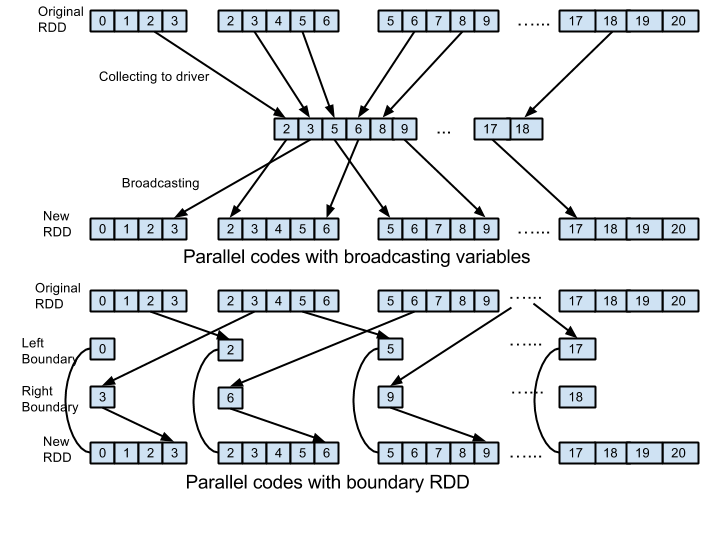
\includegraphics[scale=.6]{figures/JacobiCode.png}
\caption{Data Flow of Jacobi Parallel Codes}
\label{JacobiCode}
\end{figure}
%%%%%%%%%%%%%%%%%%%%%%%%%%%%%%%%%%%%%%%%%%%%%%%%%%%%%%
